\section{August 2019}

\subsection*{Classical Mechanics}
\addcontentsline{toc}{subsection}{Classical Mechanics}

\prob{1.1}{

A reasonable model for spherical isotropic galaxies is that the gravitational potential is roughly constant close to the galactic center but decays as $r^{-1}$ at large distances.

Such a potential, known as the H\'{e}non isochrone potential, is given by
\begin{align}
    \Phi(r) = -\frac{G M}{b + (b^2 + r^2)^{1/2}}
,\end{align}
where $G$ is the gravitational constant, $M$ is the mass of the galaxy, and $b$ is its ``size''.

\begin{parts}

\item Calculate the velocity of a star in a circular orbit of radius $R$.
It may be easier to introduce the quantity $a \equiv \sqrt{b^2 + r^2}$.

\item For all orbits, even the non-circular ones, is the angular momentum $L$ conserved?
Why?

\item For the isochrone potential, the orbits are not closed.
However, if you define the period $T_r$ as twice the time between perigee (closest distance to center) and apogee (farthest distance to center), show that, for a star of energy $E$, it is given by
\begin{align}
    T_r = \frac{2 \pi G M}{(-2 E)^{3/2}}
,\end{align}
which does not depend on the angular momentum and has the same dependence on the energy as in the Kepler problem with the inverse square law.
This is the reason this potential is called the isochrone potential.

You may find it easier if you make the change of variable $r = b(s^2 - 2s)^{1/2}$, with $s > 2$.
    
\end{parts}

\textbf{Hint}:
\begin{align}
    \int_{s_1}^{s_2} \frac{(s-1) \dd{s}}{\sqrt{(s_2 - s)(s - s_1)}} = \pi \Bigg[ \frac{s_1 + s_2}{2} - 1 \Bigg]
\end{align}

}

\sol{}


\prob{1.2}{

A particle moves in a central potential $V(r) = -V_0 e^{-\lambda^2 r^2}$.

\begin{parts}

\item Given the angular momentum $L$, find the radius of the stable circular orbit.
An implicit equation is fine.

\item It turns out that if $L$ is too large, then no circular orbit exists.
What is the largest value of $L$ for which a circular orbit does in fact exist?
    
\end{parts}

}

\sol{}


\prob{1.3}{

A uniform ladder of mass $M$ and length $L$ is placed with one end against a frictionless wall and the other end on a frictionless floor.
The ladder initially makes and angle $\theta_0$ with the floor, as shown below.

\begin{center}
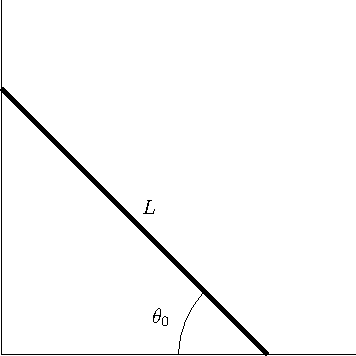
\includegraphics{August2019/1-3.pdf}
\end{center}

The ladder is released, and slides under the influence of gravity.

\begin{parts}

\item Write the Lagrangian for the sliding ladder as a function of $\theta$ (the angle of the ladder with respect to the floor).

\item At what angle $\theta$ does the ladder lose contact with the wall?
    
\end{parts}

(Note: The moment of inertia of a uniform rod of mass $M$ and length $L$ rotating about an axis through its center of mass is $I = \frac{1}{12} M L^2$)

}

\sol{}


\prob{1.4}{

Two balls of mass $m_1$ and $m_2$ are connected by a spring with an elastic constant $k$.
A third ball of mass $m$ moving with a velocity $v$ from left hits a ball 1 and gets instantly stuck to it, as shown in the figure below.
Assuming that the balls 1 and 2 were initially at rest and can slide without friction only along the $x$-axis, calculate the amplitude and frequency of oscillations after the impact.

\begin{center}
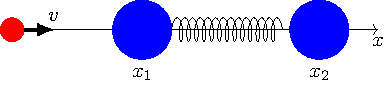
\includegraphics{August2019/1-4.pdf}
\end{center}

}

\sol{}


\prob{2.1}{

A bead of mass $m$ in a uniform gravitational field along the $z$-axis is constrained to slide without friction along a wire of parabolic shape described by $z = c \rho^2$.
The wire rotates about the $z$-axis with constant angular velocity $\omega$.
Use the method of Lagrange multipliers to find the equation of motion for the bead and expressions for the Lagrange multipliers.
What does each of the multipliers represent?

\begin{center}
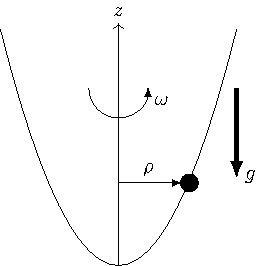
\includegraphics{August2019/2-1.pdf}
\end{center}

}

\subsection*{Electricity \& Magnetism}
\addcontentsline{toc}{subsection}{Electricity \& Magnetism}

\prob{2.2}{

A non-relativisitic particle of mass $m$ and charge $q$ moves in a magnetic field $H$ applied along the $z$-axis and a perpendicular electric field $E$ applied along the $y$ axis.
At $t = 0$ the initial velocity of the particle $\vb*{v}(0) = (v_x,0,v_z)$ has two components $v_x$ and $v_z$ directed along the $x$ and $z$ axis, respectively.

\begin{parts}

\item Calculate the coordinates of the particle $x(t)$, $y(t)$, and $z(t)$ as functions of the time at $t > 0$, if at $t = 0$ the particle was at the point $x = y = z = 0$.

\item Describe the trajectory of the particle, and calculate the direction and the magnitude of the mean drift velocity in the $xy$-plane.

\end{parts}

}

\sol{}


\prob{2.3}{

A thin circular ring of radius $R$ lies in the $xy$-plane with its center at the origin $x = 0$, $y = 0$.
The ring consists of two half-rings that are homogeneously charged and have opposite total charges $+q$ and $-q$.

Find the electrostatic potential $\Phi(x,y,z)$ and the electrostatic field $\vb*{E}(x,y,z)$ on the $z$-axis, i.e. in the region $x^2 + y^2 \ll R^2$.

Calculate the electric field at large distances $x^2 + y^2 + z^2 \equiv r^2 \gg R^2$.

}

\sol{}


\prob{2.4}{

A far away galaxy emits 2 jets of material with identical speed $\beta c$ in opposite directions at an angle $\theta$ to the direction of the earth.

The jets include singly-ionized Mg that emits radiation with a proper wavelength $\lambda_0 = 448.1~{\rm nm}$.

From the earth the Mg lines are observed to have the wavelengths $\lambda_+ = 728.2~{\rm nm}$ and $\lambda_- = 392.1~{\rm nm}$.

Assume that the velocity of the galaxy with respect to the earth is negligible.

\begin{parts}

\item Show that the Doppler-shifted frequencies are
\begin{align}
    \omega_{\pm} = \frac{\omega_0}{\gamma(1 \pm \beta \cos{\theta})}
.\end{align}

\item Calculate $\beta$ and $\theta$.
    
\end{parts}

}

\sol{}


\prob{3.1}{

Two semi-infinite grounded conducting plates meet at right angles.
How much work does it take to bring a point charge from infinity to the point located at a distance $a$ from the first plate and distance $b$ from the second?

}

\sol{}


\prob{3.2}{

A $\Lambda^{*}(1520)$ hyperon with a mass $M_{\Lambda^*} = 1520~{\rm MeV}$ decays into a proton with $M_p = 938~{\rm MeV}$ and a negative kaon, $K^-$, with $M_K = 500~{\rm MeV}$.
Find the momentum of the kaon in the rest frame of $\Lambda^{*}(1520)$.

}

\sol{}


\prob{3.3}{

A particle with rest mass $mc^2$ and energy $E$ approaches an identical particle at rest.
They collide elastically (i.e., none of the rest masses change) in such a way that they both scatter at an angle $\theta$ relative to the incident direction.
What is $\theta$ in terms of $E$ and $mc^2$?
What is $\theta$ at $E \gg mc^2$ and $E \simeq mc^2$, i.e., in the extreme relativistic and non-relativistic limits?

}

\subsection*{Quantum Mechanics}
\addcontentsline{toc}{subsection}{Quantum Mechanics}


\prob{3.4}{

Consider a particle in the infinitely deep potential well of width $a$, i.e.,
\begin{align}
    U(x) = \begin{cases}
        0 & 0 < x < a \\
        \infty & x < 0, x > a
    .\end{cases}
\end{align}

\begin{parts}

\item Find the normalized wave functions of stationary levels in the coordinate $\Psi_n(x)$ and momentum $\widetilde{\Psi}_n(p)$ representations and the energies of these levels.

\item Draw $|\Psi_n(x)|^2$ and $|\widetilde{\Psi}_n(p)|^2$ for the two lowest levels.

\item For the $n^{\rm th}$ energy level, find the averages $\expval{x}$, $\expval{p}$, $\Delta x^2$, and $\Delta p^2$.

\item Check that the uncertainty relation $\Delta x \Delta p \geq \hbar / 2$ holds for each energy level.
    
\end{parts}

}

\sol{}


\prob{4.1}{

Consider a spin-1/2 particle confined to move in the $xy$-plane and described by the Hamiltonian
\begin{align}
    H = \frac{\hat{p}^2}{2m} + \alpha(\hat{p}_y \hat{\sigma}_x - \hat{p}_x \hat{\sigma}_y) + \beta(\hat{p}_x \hat{\sigma}_x - \hat{p}_y \hat{\sigma}_y) + \mu B \hat{\sigma}_z
,\end{align}
where $\hat{\vb*{p}}$ is the momentum operator, and $\hat{\sigma}$ are the Pauli matrices.
The second and the third terms in $\hat{H}$ describe spin-orbital interaction quantified by the real coupling constants $\alpha$ and $\beta$, and the last term is the Zeeman energy of the magnetic field $B$ applied along the $z$-axis.

Diagonalize the Hamiltonian $H$ and calculate its eigenvalues.

}

\sol{}


\prob{4.2}{

Two atoms with $j_1 = 1$ and $j_2 = 2$ are coupled, with an energy described by $H = a \vb*{J}_1 \cdot \vb*{J}_1$ ($a > 0$).
Determine all possible energies and degeneracies for the coupled system.
What are the eigenstates corresponding to maximal and minimal energy.

}

\sol{}


\prob{4.3}{

Consider an electron of mass $m$ and charge $q$ moving on the surface of a liquid helium.
Assume the liquid helium surface is the plane $xOy$ with $z < 0$ inside the liquid.

The potential between the electron and the liquid helium is assumed to be infinite inside the liquid.
Above the liquid the electron experiences an electrostatic potential given by
\begin{align}
    V(z) = -\frac{\Lambda}{z},~{\rm with}~ \Lambda = \frac{q^2}{4 \pi \epsilon_0} \frac{\epsilon - 1}{4(\epsilon + 1)}
,\end{align}
where $\epsilon$ is the dielectric constant of liquid helium.

Assume that the wave function of the electron is $\Psi_1(z > 0) = c1 z \exp(-\kappa_1 z)$ with $c_1$ and $\kappa_1$ positive real numbers.

\begin{parts}
    
\item Determine the coefficient $\kappa_1$ and the energy $E_1$.
Express them as functions of $m$, $\Lambda$, and $\hbar$.

\item Is $\Psi_1(z)$ the lowest energy state of the electron? Why?

\item Calculate the constant $c_1$ and determine the mean distance $\expval{z}$ of the electron above the surface when it is in state $\Psi_1(z)$.
Express it as function of $m$, $\Lambda$, and $\hbar$.

Assume now that the electron is in the state described by the wave function $\Psi_2(z > 0) = c_2(1 - \kappa_2 z) \exp(-\kappa_2 z)$ with $c_2$ and $\kappa_2$ positive real numbers.

\item Determine the coefficient $\kappa_2$ and the energy $E_2$.
Express them as functions of $m$, $\Lambda$, and $\hbar$.

Check that $E_2 = E_1 / 4$.

\item Is $\Psi_2(z)$ the first excited state of the electron? Why?

\end{parts}

\textbf{Hint}: $\int_0^\infty u^n e^{-nu} \dd{u} = n!$

}

\sol{}


\prob{4.4}{

Use the momentum representation to calculate the ground state of a particle in an attractive one-dimensional potential, which in the coordinate representation is given by $W(x) = -c\delta(x)$ ($c > 0$).

}
